\chapter{Indoor Localization}

We usually take the localization for granted, but it is a very complex problem, especially in indoor environments.

For outdoor is much easier, since we can use GPS.

\textbf{Relative location}, may be turned in \textbf{absolute location} if the reference points absolute location is known, or if multiple relative readings and fusion strategy are available.

GNSS (Global Navigation Satellite System) is the most common outdoor localization system, and includes:
\begin{itemize}
   \item GPS (USA)
   \item GLONASS (Russia)
   \item Galileo (EU)
   \item Beidou (China)
\end{itemize}

\section*{Indoor Localization Systems}
Currently this is an open research issue, typically solved by means of ad hoc solutions.

It is incredibly various, in terms of:
\begin{itemize}
   \item \textbf{Signal types}
   \item \textbf{Signal metrics}
   \item \textbf{Metric processing methods}
\end{itemize}

\section{Signal Types}
\begin{itemize}
   \item Infrared
   \item UWB
   \item Ultrasound
   \item WiFi
\end{itemize}

\begin{figure}[htbp]
   \centering
   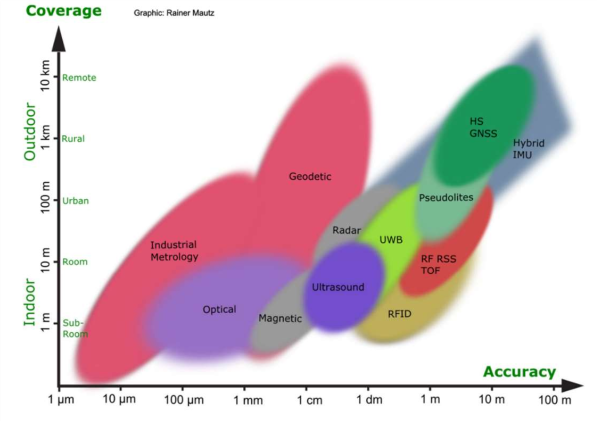
\includegraphics{images/signaltypes.png}
   \caption{Signal types graph}
   \label{fig:signaltypes}
\end{figure}
\section{Signal Metrics}
There are three main ranging approaches which exploit different signal metrics:
\begin{itemize}
   \item \textbf{Time} based
   \item \textbf{Angle} based
   \item[] These two are the most common, but work only if transmitters and measuring units are in LOS (Line of Sight)
   \item Received Signal \textbf{Indicators} based
\end{itemize}

\subsection{ToA - Time of Arrival}
The distance between a measuring unit and a mobile target is directly proportional to the propagation time.\\
Mathematically speaking, being $p$ the propagation speed, $t$ the time of transmission and $t'$ the time of reception, the distance $d$ is:
\[
   d = (t' - t) \cdot p
\]
This method requires a tight synchronization of transmitter and receiver, and that the signal encodes the transmission time $t$.\\
Besides, to compute the position in a plane (2D), at least 3 anchors ---located in different positions--- are needed.

In some applications, ToA is implemented by two types of signals, an Acoustic signal and a Radio one.
The radio, since it is order of magnitude faster than the acoustic signal, is used to synchronize the measuring units, while the acoustic signal is used to measure the distance.

\subsection{TDoA - Time Difference of Arrival}
The distance between a measuring unit and a mobile target is directly proportional to the difference in propagation time between two signals.

The hyperbolic location theory is:
The hyperbola is the set of points at a constant range-difference $c\cdot\Delta t$ from two foci (?).
Each sensor pair gives a hyperbola on which the emitter lies.
Location estimation is the intersection of all hyperbolas.

\begin{figure}[htbp]
   \centering
   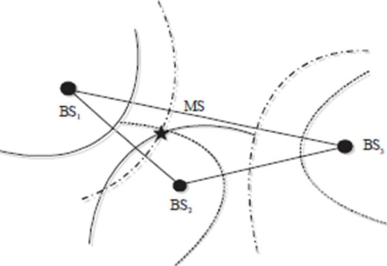
\includegraphics{images/tdoa.png}
   \caption{TDoA example}
   \label{fig:tdoa}
\end{figure}

\subsection{RTOF - Round Trip Time of Flight}
The transmitter and the measuring unit are the same. The device to be localized is only a transponder, i.e. receives the signal and sends it back.
\[
   distance = c\cdot(t_1 - t_2)/2
\]
This requires much less synchronization compared to ToA, but the signal must be able to be received and sent back.

\subsection{AoA - Angle of Arrival}

There are some antennas which allow to measure the angle of arrival of a signal, and this can be used to estimate the position of the emitter.\\
2D localization requires at least 2 antennas, while 3D localization requires at least 3 antennas.

AoA is more expensive and usually not available in sensors. Besides, it is very sensitive to the environment, multipath and reflection may affect the measurement.

\section{Signal Processing}
Processing methods may be \textbf{Range-free} or \textbf{Range-based}.

\subsection{Range-free}
One of the most common range-free methods is the \textbf{Centroid}. 
The idea, is to do not use any ranging at all, but simply
deploy enough anchors periodically broadcasting their
location.
The algorithm is simple and based on listening to anchors, but their positioning is crucial.
\nl

DV-Hop is a range-free localization algorithm, which uses the distance between nodes to estimate the position of the nodes.
\begin{itemize}
   \item Anchors:
   \begin{itemize}
      \item Flood network with known positions
      \item Flood network with average hop distance
   \end{itemize}
   \item Nodes:
   \begin{itemize}
      \item Count $\#hops$ to anchors
      \item Multiply with avg hop distance
   \end{itemize}
\end{itemize}
\nl

In APIT (Approximate Point In Triangle test) anchors divide the environment into triangular regions:
a node's presence inside or outside of these triangular regions allows to narrow the area in which it can potentially reside.

\subsection{Range-based}
\textbf{Multilateration} is a range-based method, which uses the distance between the measuring unit and the anchors to estimate the position of the measuring unit.

The node collects the beacons and estimate its distance to each beacon.

\begin{figure}[htbp]
   \centering
   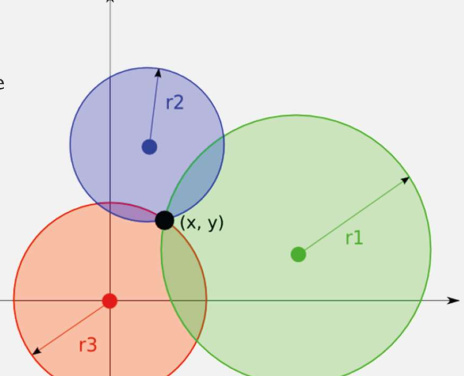
\includegraphics{images/multilateration.png}
   \caption{Multilateration example}
   \label{fig:multilateration}
\end{figure}
\nl

In MIN-MAX a node creates an association between each anchor position and the strength of the RSS from that anchor.
By inverting the nominal distance-power loss law, the node may estimate his distance from each beacon
\begin{figure}[htbp]
   \centering
   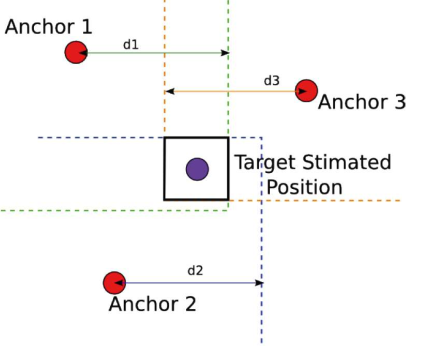
\includegraphics{images/minmax.png}
   \caption{MinMax algorithm in the plane}
   \label{fig:minmax}
\end{figure}

TODO

\subsection{TODO}

\href{filippo.palumbo@isti.cnr.it}{filippo.palumbo@isti.cnr.it}
